%\begin{documment}

\begin{figure}[t]
\begin{lstlisting}%[backgroundcolor=\color{white}]

// DECLARATIONS
input <type> <id>;      // external event
event <type> <id>;      // internal event
var   <type> <id>;      // variable

// EVENT HANDLING
await <id>;             // awaits event
emit  <id>;             // emits  event

// COMPOUND STATEMENTS
<...> ; <...> ;         // sequence
if <...> then <...>     // conditional
         else <...> end
loop do <...> end       // repetition
    break               //   (escape loop)
finalize <...>          // finalization
    with <...> end

// PARALLEL COMPOSITIONS
par/and do <...>        // rejoins on termination of both sides
      with <...> end
par/or do  <...>        // rejoins on termination of any side
      with <...> end
par do <...>            // never rejoins
  with <...> end

// C INTEGRATION
_f();                   // C call (prefix `_')
native do <...> end     // block of native code
pure <id>;              // pure annotation
safe <id> with <id>;    // safe annotation
\end{lstlisting}
\rule{14cm}{0.37pt}
\caption{ Syntax of \CEU.\newline
{\small %\textmd{
}%}
\label{lst.syntax}
}
\end{figure}

\CEU is a concurrent language in which multiple lines of execution---known as 
\emph{trails}---continuously react to input events from the environment.
Waiting for an event halts the running trail until that event occurs.
The environment broadcasts an occurring event to all active trails, which share 
a single global time reference (the event itself).
%
%\section{Parallel syntactic compositions}
%\label{sec.ceu.par}
%
The fundamental distinction between \CEU and prevailing multi-threaded designs 
is the way threads are combined in programs.
\CEU provides Esterel-like syntactic hierarchical compositions, while most 
multi-threaded systems typically only support top-level definitions for threads 
(i.e., they cannot be nested).
Figure~\ref{lst.syntax} shows a compact reference of the syntax of \CEU, which 
helps to follow the examples in this chapter.
%\CEU distinguishes itself from Esterel by its tight integration with $C$ and 
%support for shared memory, which also demands an effective safety analysis 
%permeating (and affecting) all language features.

We start the chapter with the fundamental design decisions behind \CEU's 
execution model, namely the uniqueness of external events and deterministic 
scheduler (Section~\ref{sec.ceu.det}).
Then, we discuss how they enable safe concurrency support for shared memory and 
native $C$ function calls (Sections~\ref{sec.ceu.shared}~and~\ref{sec.ceu.c}).
%
%We follow with discussion about a key characteristic of synchronous languages: 
%activities in parallel that support nesting and abortion 
%(Section~\ref{sec.ceu.par}).
%
We further introduce some new programming features that match \CEU's 
synchronous and safety-oriented design:
local scope finalization (Section~\ref{sec.ceu.fins}),
first-class timers (Section~\ref{sec.ceu.wclocks}),
and a stack-based communication mechanism (Section~\ref{sec.ceu.ints}).
%
We finish with a discussion that summarizes the chapter by comparing \CEU with 
Esterel (Section~\ref{sec.ceu.esterel}).

\section{The execution model of C\'eu}
\label{sec.ceu.det}

% TODO: motivate?

\CEU is grounded on a precise definition of ``logical time'' as a discrete 
sequence of external input events:
% \footnote{We use the terms \emph{external input event}, \emph{external event}, 
%and \emph{input event} interchangeably.}
a sequence because only a single input event is handled at a logical time; 
discrete because reactions to events are guaranteed to execute in bounded time 
(here the ``physical'' notion of time, to be discussed further).
The execution model for \CEU programs is as follows:

\begin{enumerate}
\item The program initiates the ``boot reaction'' in a single trail.
\item Active trails execute until they await or terminate.
      This step is named a \emph{reaction chain}, and always runs in bounded 
      time.
\item The program goes idle and the environment takes control.
\item On the occurrence of a new external input event, the environment awakes 
      \emph{all} trails awaiting that event.
      It then goes to step 2.
\end{enumerate}

% TODO
The synchronous execution model of \CEU is based on the hypothesis that 
internal reactions run \emph{infinitely faster} in comparison to the rate of 
external events~\cite{rp.hypothesis}.
An internal reaction is the set of computations that execute when an external 
event occurs.
Conceptually, a program takes no time on step 2 and is always idle on step 3.
In practice, if a new external input event occurs while a reaction chain is 
running (step 2), it is enqueued to run in the next reaction.
%, because reaction chains must run to completion.
%
% TODO: a similar approach is taken in \cite{...}
%
When multiple trails are active at a logical time (i.e. awaking on the same 
event), \CEU schedules them in the order they appear in the program text.
This policy is somewhat arbitrary, but provides a priority scheme for trails, 
and also ensures deterministic and reproducible execution for programs, which 
is important for simulation purposes.
A reaction chain may also contain emissions and reactions to internal events, 
which are presented in Section~\ref{sec.ceu.ints}.

The synchronous model is applicable to typical WSN applications, which are most 
of the time waiting for events (e.g. timers and network packets) to perform a 
fast reaction (e.g. forwarding a packet or blinking a LED) before going idle 
again.

\begin{figure}[h]
\begin{lstlisting}[numbers=left,xleftmargin=2em]
input void A, B, C;
par/and do
    // trail 1
    <...>         // <...> represents non-awaiting statements
    await A;
    <...>
with
    // trail 2
    <...>
    await B;
    <...>
with
    // trail 3
    <...>
    await A;
    <...>
    await B;
    par/and do
        // trail 3
        <...>
    with
        // trail 4
        <...>
    end
end
\end{lstlisting}
%
\rule{14cm}{0.37pt}
\caption{ A \CEU program to illustrate the scheduler behavior.
{\small %\textmd{
}%}
\label{lst.reaction}
}
\end{figure}

\begin{figure}[h]
\centering
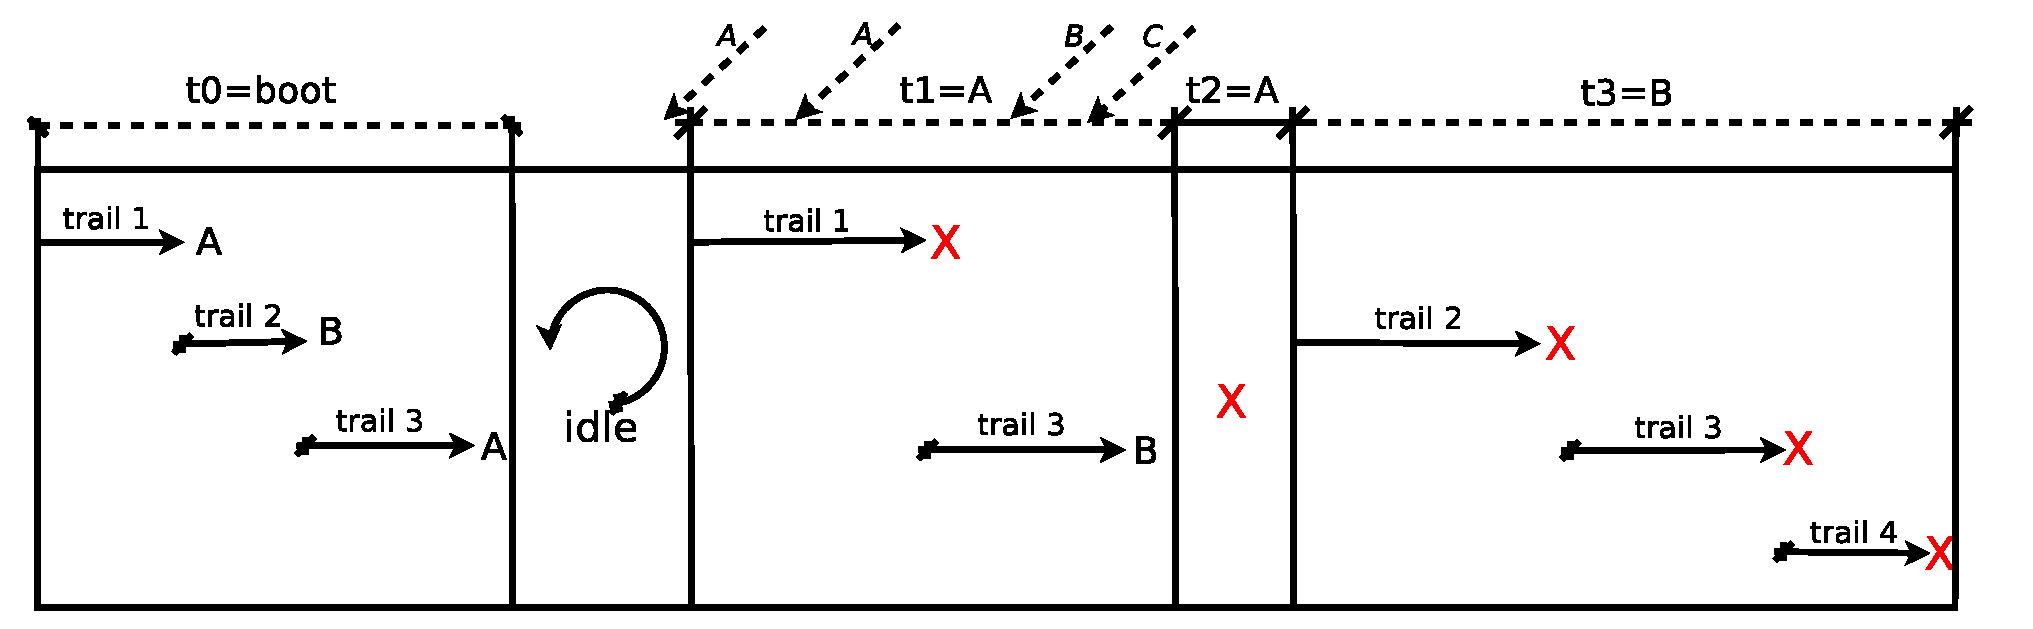
\includegraphics[scale=0.45]{reaction}
\caption{ A sequence of reaction chains for the program in 
Figure~\ref{lst.reaction}.
\label{fig.reaction}
}
\end{figure}

To illustrate the behavior of the scheduler of \CEU, the execution of the 
program in Figure~\ref{lst.reaction} is depicted in the diagram of 
Figure~\ref{fig.reaction}.
%
The program starts in the boot reaction and is split in three trails.
Following the order of declaration, the scheduler first executes \emph{trail~1} 
until it awaits $A$ in line 5;
then \emph{trail~2} executes until it awaits $B$ in line 10;
then \emph{trail~3} is scheduled and also awaits $A$, in line 15.
%
As no other trails are pending, the reaction chain terminates and the scheduler 
remains idle until the occurrence of $A$:
\emph{trail~1} awakes, executes and terminates;
and then \emph{trail 3} executes and waits for $B$ in line 17.
\emph{Trail~2} remains suspended, as it is not awaiting $A$.
%
During this reaction, new instances of events $A$, $B$, and $C$ occur and are 
enqueued to be handled in the reactions that follow.
%
As $A$ happened first, it is used in the next reaction.
However, no trails are awaiting it, so an empty reaction chain takes place.
%
The next reaction dequeues event $B$:
\emph{trail 2} awakes, executes and terminates;
then \emph{trail 3} is split in two and both terminate.
%
The program terminates and does not react to the pending event $C$.
% (the \code{par/and}, to be introduced in the next section, rejoins when its 
%sub-trails terminate).
%
Note that each step in the logical time line ($t0$, $t1$, etc.) is identified 
by the event it handles.
Inside a reaction, trails only react to that identifying event (or remain 
suspended).

\subsection{Bounded execution}

Reaction chains should run in bounded time to guarantee that programs are 
responsive and can handle upcoming input events from the environment.
Similarly to Esterel~\cite{esterel.ieee91}, \CEU requires that each possible 
path in a loop body contains at least one \code{await} or \code{break} 
statement, thus ensuring that loops never run in unbounded time.
%
Consider the examples that follow:

\nopagebreak
\noindent
\begin{minipage}[t]{0.45\linewidth}
\begin{lstlisting}
loop do
    if <cond> then
        break;
    end
end
\end{lstlisting}
\end{minipage}
%
\begin{minipage}[t]{0.45\linewidth}
\begin{lstlisting}
loop do
    if <cond> then
        break;
    else
        await A;
    end
end
\end{lstlisting}
\end{minipage}

The first example is refused at compile time, because the \code{if} true branch 
may never execute, resulting in a \emph{tight loop} (i.e., an infinite loop 
that does not await).
The second variation is accepted, because for every iteration, the loop either 
breaks or awaits.

Enforcing bounded execution makes \CEU inappropriate for algorithmic-intensive 
applications that require unrestricted loops (e.g., cryptography, image 
processing).
However, \CEU is designed for control-intensive applications and we believe 
this is a reasonable price to pay in order to achieve higher reliability.
%
We evaluate the responsiveness of the radio driver when this restriction is 
(intentionally) relaxed and discuss alternatives adopted in other synchronous 
languages in Section~\ref{sec.eval.radio}.

\subsection{Parallel compositions and abortion}
\label{sec.ceu.par}

The use of trails in parallel allows that programs wait for multiple events at 
the same time.
Furthermore, trails await without loosing context information, such as locals 
and the program counter, what is a desired behavior in concurrent 
applications.~\cite{sync_async.cooperative}

\CEU supports three kinds of parallel constructs regarding how they rejoin in 
the future:
a \code{par/and} requires that all trails in parallel terminate before 
proceeding to the next statement;
a \code{par/or} requires that any trail in parallel terminates before 
proceeding to the next statement, aborting all awaiting sibling trails;
finally, a \code{par} never rejoins and should be used when trails in parallel 
are supposed to run forever (if all trails in \code{par} terminates, the 
scheduler forcedly halts them forever).
%
To illustrate how trails rejoin, consider the two variations of the following 
archetype:

\begin{minipage}[t]{0.40\linewidth}
\begin{lstlisting}
loop do
    par/and do
        <...>
    with
        await 100ms;
    end
end
\end{lstlisting}
\end{minipage}
%
\begin{minipage}[t]{0.40\linewidth}
\begin{lstlisting}
loop do
    par/or do
        <...>
    with
        await 100ms;
    end
end
\end{lstlisting}
\end{minipage}

In the \code{par/and} variation, the block marked as \code{<...>} in the first 
trail (which may contain nested compositions with \code{await} statements) is 
repeated every $100$ milliseconds at minimum, as both sides must terminate 
before re-executing the loop.
In the \code{par/or} variation, if the block does not terminate within $100$ 
milliseconds, it is restarted.
These archetypes represent, respectively, the \emph{sampling} and 
\emph{timeout} patterns, which are very common in reactive applications.

The code in Figure~\ref{lst.radio} is extracted from our implementation of the 
\emph{CC2420} radio driver and uses a \code{par/or} to control the start/stop 
behavior of the radio.
The input events \code{CC2420\_START} and \code{CC2420\_STOP} (line 1) 
represent the external interface of the driver with a client application (e.g.  
a protocol).
The driver enters the top-level loop and awaits the starting event (line 3);
once the client application makes a start request, the driver spawns two other 
trails:
one to await the stopping event (line 5),
and another to actually receive radio messages in a loop (collapsed in line 9).
%
As compositions can be nested, the receiving loop can be as complex as needed, 
including other loops and parallel constructs.
However, once the client requests to stop the driver, the trail in line 5 
awakes and terminates, causing the \code{par/or} also terminate and abort the 
receiving loop.
In this case, the top-level loop restarts and waits for the next request to 
start the radio (line 3, again).

\begin{figure}[t]
\begin{lstlisting}[numbers=left,xleftmargin=2em]
input void CC2420_START, CC2420_STOP;
loop do
    await CC2420_START;
    par/or do
        await CC2420_STOP;
    with
        // loop with other nested trails
        // to receive radio packets
        <...>
    end
end
\end{lstlisting}
\rule{14cm}{0.37pt}
\caption{ Start/stop behavior for the radio driver.\newline
{\small %\textmd{
The occurrence of \code{CC2420\_STOP} (line 5) seamlessly aborts the receiving 
loop (collapsed in line 9) and resets the driver to wait for the next 
\code{CC2420\_START} (line 3).
}%}
\label{lst.radio}
}
\end{figure}

The \code{par/or} construct of \CEU is regarded as an \emph{orthogonal 
preemption primitive}~\cite{esterel.preemption} because the two sides in the 
composition need not be tweaked with synchronization primitives or state 
variables in
order to affect each other.
In contrast, it is known that traditional (asynchronous) multi-threaded 
languages cannot express thread abortion 
safely~\cite{esterel.preemption,sync_async.threadsstop}.
For instance, it is not safe to terminate a thread holding a lock.

\subsection{Reasoning about concurrency}

The blinking LED of Figure~\ref{lst.all} in \CEU illustrates how synchronous 
parallel constructs lead to a simpler reasoning about concurrency aspects in 
comparison to the other implementations.
As reaction times are assumed to be instantaneous, the blinking loop takes 
exactly 3 seconds (i.e., $2s+1s$).
Hence, after 20 iterations, the accumulated time becomes 60 seconds and the 
loop terminates concurrently with the 1-minute timeout in parallel.
Given that the loop appears first in the code, the scheduler will restart it 
and turn on the LED for the last time.
Then, the 1-minute timeout is scheduled, aborts the whole \code{par/or}, and 
turns off the LED.
%
This reasoning is actually reproducible in practice, and the LED will light on 
exactly 21 times for every single execution of this program.
First-class timers are discussed in more detail in 
Section~\ref{sec.ceu.wclocks}.
%
Note that this static control inference is impossible in asynchronous 
languages, given that internal reactions take an unpredictable time (as 
illustrated in Figure~\ref{lst.related.leds}).
Even in the other implementations of Figure~\ref{lst.all}, this control 
inference cannot be easily extracted, specially considering the presence of two 
different timers.

The behavior for the LED timeout just described denotes a \emph{weak abortion}, 
because the blinking trail had the chance to execute for the last time.
By inverting the two trails, the \code{par/or} would terminate immediately, and 
the blinking trail would not execute, denoting a \emph{strong 
abortion}~\cite{esterel.preemption}.
%
\CEU not only provides means to choose between weak and strong abortion, but 
also detects the two conflicting possibilities and issues a warning at compile 
time (to be discussed in Section~\ref{sec.ceu.shared}).

% TODO: pause

\section{Shared-memory concurrency}
\label{sec.ceu.shared}

WSN applications make extensive use of shared memory, such as for handling 
memory pools, message queues, routing tables, etc.
Hence, an important goal of \CEU is to ensure a reliable execution for 
concurrent programs that share memory.
%
Concurrency in \CEU is characterized when two or more trail segments in 
parallel execute during the same reaction chain.
A trail segment is a sequence of statements followed by an \code{await} (or 
termination).

In the first code fragment that follows, the two assignments to \code{x} run 
concurrently, because both trail segments are spawned during the same reaction 
chain.
However, in the second code fragment, the assignments to \code{y} are never 
concurrent, because \code{A} and \code{B} are different external events and the 
respective segments can never execute during the same reaction chain:

\nopagebreak
\noindent
\begin{minipage}[t]{0.45\linewidth}
\begin{lstlisting}
var int x=1;
par/and do
    x = x + 1;
with
    x = x * 2;
end
\end{lstlisting}
\end{minipage}
%
\begin{minipage}[t]{0.45\linewidth}
\begin{lstlisting}
input void A, B;
var int y=0;
par/and do
    await A;
    y = y + 1;
with
    await B;
    y = y * 2;
end
\end{lstlisting}
\end{minipage}

Note that although the variable \code{x} is accessed concurrently in the first 
example, the assignments are both atomic and deterministic: the final value of 
\code{x} is always $4$ (i.e. {\small$(1+1)*2)$}).
%
Remember from Section~\ref{sec.ceu.det} that trails are scheduled in the order 
they appear and run to completion (i.e., until they await or 
terminate).
%
However, programs with concurrent accesses to shared memory are suspicious, 
because an apparently innocuous reordering of trails modifies the semantics of 
the program; for instance, the previous example would yield $3$ with the trails 
reordered, i.e., {\small$(1*2+1)$}.

%Moreover, \CEU also supports pointers, which are required for low-level 
%manipulation (e.g., accessing buffers from device drivers).

We developed a compile-time temporal analysis for \CEU in order to detect 
concurrent accesses to shared variables, as follows:
\emph{if a variable is written in a trail segment, then a concurrent trail 
segment cannot read or write to that variable, nor dereference a pointer of 
that variable type.}
An analogous policy is applied for pointers \emph{vs} variables and pointers 
\emph{vs} pointers.
The algorithm for the analysis holds the set of all events in preceding 
\code{await} statements for each variable access.
Then, the sets for all accesses in parallel trails are compared to assert that 
no events are shared among them.
Otherwise the compiler warns about the suspicious accesses.

Consider the three examples in Figure~\ref{lst.det}.
The first code is detected as suspicious, because the assignments to \code{x} 
and \code{p} (lines 11 and 14) may be concurrent in a reaction to \code{A} 
(lines 6 and 13);
%
In the second code, although two of the assignments to \code{y} occur in 
reactions to \code{A} (lines 4-5 and 10-11), they are not in parallel trails 
and, hence, are safe.
Note that the assignment in reaction to \code{B} (line 8) is safe given that 
reactions to different events cannot overlap (due to the single-event rule).
%
The third code illustrates a false positive in our algorithm: the assignments 
to \code{z} in parallel can only occur in different reactions to \code{A} 
(lines 5 and 9), as the second assignment awaits two occurrences of \code{A}, 
while the first trail assigns and terminates in the first occurrence.

We also implemented an alternative algorithm that converts a \CEU program into 
a deterministic finite automata.
The resulting DFA represents all possible points a program can reach during 
runtime and, hence, eliminates all false positives.
However, the algorithm is exponential and may be impractical in some 
situations.
%
For this reason, we opted for the simpler algorithm.
%
That being said, the simpler static analysis does not detect false positives in 
any of the
implementations to be presented in Section~\ref{sec.eval} and executes in 
negligible time, suggesting that the algorithm is practical.

\begin{figure}[t]
\begin{minipage}[t]{0.39\linewidth}
\begin{lstlisting}[numbers=left,xleftmargin=2em]
input void A;
var int x;
var int* p;
par/or do
  loop do
    await A;
    if <cnd> then
      break;
    end
  end
  x = 1;
with
  await A;
  *p = 2;
end

\end{lstlisting}
\end{minipage}
%
%
\begin{minipage}[t]{0.33\linewidth}
\begin{lstlisting}
input void A, B;
var int y;
par/or do
  await A;
  y = 1;
with
  await B;
  y = 2;
end
await A;
y = 3;

\end{lstlisting}
\end{minipage}
%
%
\begin{minipage}[t]{0.25\linewidth}
\begin{lstlisting}
input void A;
var int z;
par/and do
  await A;
  z = 1;
with
  await A;
  await A;
  z = 2;
end
\end{lstlisting}
\end{minipage}
%
\rule{14cm}{0.37pt}
\caption{ Automatic detection for concurrent accesses to shared memory. \newline
{\small %\textmd{
The first example is suspicious because \code{x} and \code{p} can be accessed 
concurrently (lines 11 and 14).
The second example is safe because accesses to \code{y} can only occur in 
sequence.
The third example illustrates a false positive in our algorithm.
}%}
\label{lst.det}
}
\end{figure}

Conflicting weak and strong abortions, as introduced in 
Section~\ref{sec.ceu.det}, are also detected with the proposed algorithm.
Besides accesses to variables, the algorithm also keeps track of trail 
terminations inside a \code{par/or}, issuing a warning when they can occur 
concurrently.
This way, the programmer can be aware about the conflict existence and choose
between weak or strong abortion.

The proposed static analysis is only possible due to the uniqueness of external 
events within reactions and support for syntactic compositions, which provide 
precise information about the flow of trails (i.e., which run in parallel and 
which are guaranteed to be in sequence).
Such precious information cannot be inferred when the program relies on state 
variables to handle control, as typically occurs in event-driven systems.

\section{Integration with $C$}
\label{sec.ceu.c}

Most existing operating systems and libraries for WSNs are based on $C$, given 
its omnipresence and level of portability across embedded platforms.
Therefore, it is fundamental that programs in \CEU have access to all 
functionality the underlying platform already provides.

In \CEU, any identifier prefixed with an underscore is repassed \emph{as is} to 
the $C$ compiler that generates the final binary.
Therefore, access to $C$ is seamless and, more importantly, easily trackable.
%
\CEU also supports \emph{native~blocks} to define new symbols in $C$, as 
Figure~\ref{lst.c} illustrates.
Code inside ``\code{native~do~...~end}'' is also repassed to the $C$ compiler 
for the final generation phase.
%Only global definitions are allowed inside $C$ blocks.
As \CEU{} mimics the type system of $C$, values can be easily passed back and 
forth between the languages.

% TODO: real example?
\begin{figure}[t]
\begin{lstlisting}[numbers=left,xleftmargin=2em]
native do
    #include <assert.h>
    int I = 0;
    int inc (int i) {
        return I+i;
    }
end
native _assert(), _inc(), _I;
_assert(_inc(_I));
\end{lstlisting}
%
\rule{14cm}{0.37pt}
\caption{ A \CEU program with embedded $C$ definitions.
{\small %\textmd{
The globals \code{I} and \code{inc} are defined in the \code{native} block 
(lines 3 and 4), and are imported by \CEU in line 8.
$C$ symbols must be prefixed with an underline to be used in \CEU (line 9).
}%}
\label{lst.c}
}
\end{figure}

$C$ calls are fully integrated with the static analysis presented in
Section~\ref{sec.ceu.shared} and cannot appear in concurrent trails segments, 
because \CEU has no knowledge about their side effects (e.g. calls that access 
the same LED).
Also, passing variables as parameters is regarded as read accesses to them, 
while passing pointers as write accesses to those types (because functions may 
dereference and assign to them).
%
This policy increases considerably the number of false positives in the 
analysis, given that many functions can actually be safely called concurrently.
Therefore, \CEU supports explicit syntactic annotations to relax the policy.
They are illustrated in Figure~\ref{lst.annotations}, and are described as 
follows:

\begin{itemize}
\item The \code{pure} modifier declares a $C$ function that does not cause side 
      effects, allowing it to be called concurrently with any other function in 
the program.
\item The \code{safe} modifier declares a pair of variables or functions that 
      do not affect each other, allowing them to be used concurrently.
\end{itemize}

%The following code illustrates \CEU annotations:
%
% TODO: exs from ports

\begin{figure}[t]
\begin{lstlisting}[numbers=left,xleftmargin=2em]
pure  _abs();               // side-effect free
safe _Leds_led0Toggle with  // 'led0' vs 'led1' is safe
     _Leds_led1Toggle;
var int* buf1, buf2;        // point to different buffers
safe buf1 with buf2;        // 'buf1' vs 'buf2' is safe
\end{lstlisting}
\caption{ Annotations for $C$ functions. \newline
{\small %\textmd{
Function \code{abs} is side-effect free and can be concurrent with any other 
function.
The functions \code{\_Leds\_led0Toggle} and \code{\_Leds\_led1Toggle} can 
execute concurrently.
The variables \code{buf1} and \code{buf2} can be accessed concurrently 
(annotations are also applied to variables).
}%}
\label{lst.annotations}
}
\end{figure}

\begin{comment}
TODO

Annotations are typically write-once declarations (when integrating a $C$ 
service for the first time) to be included in actual applications.
Note that the example in Figure~\ref{lst.blink} should include the annotation 
for \code{\_Leds\_led0Toggle} and \code{\_Leds\_led1Toggle} above to be 
compiled correctly.
\end{comment}

\CEU does not extend the bounded execution analysis to $C$ function calls. 
% which are left as responsibility for the programmer.
% TODO: other languages dont as well
On the one hand, $C$ calls must be carefully analyzed in order to keep programs 
responsive.
On the other hand, they also provide means to circumvent the rigor of \CEU in a 
well-marked way (the special underscore syntax).
%
\begin{comment}
This approach is also adopted by Esterel, which supports the \code{call} 
primitive to execute code assumed to be instantaneous in the host 
language~\cite{esterel.primer}.
In \CEU, we take a step further and statically detects when such calls may 
execute concurrently, as discussed in the next section.
\end{comment}
%
Evidently, programs should only resort to $C$ for simple operations that can be 
assumed to be instantaneous, such as non-blocking I/O and \code{struct} 
accessors, but never for control purposes.
% (e.g. interrupt handling).

\section{Local scopes and finalization}
\label{sec.ceu.fins}

\begin{comment}
Furthermore, system-level development typically involves accesses to the 
underlying platform through $C$ system calls that hold pointers for some time
(e.g. transmission of a message buffer).
Hence, if a local variable goes out of scope and its reference has been 
exposed, a system-level activity may end up with a dangling pointer (i.e. a 
pointer to a freed memory).
\end{comment}

Local declarations for variables bring definitions closer to their use in 
programs, increasing the readability and containment of code.
Another benefit, specially in the context of WSNs, is that blocks in sequence 
can share the same memory space, as they can never be active at the same time.
%
The syntactic compositions of trails allow the \CEU compiler to statically 
allocate and optimize memory usage:
%, as also proposed in other systems~\cite{wsn.osm,wsn.ocram}:
memory for trails in parallel must coexist;
trails that follow rejoin points reuse all memory.

However, the unrestricted use of locals may introduce subtle bugs when dealing 
with pointers and $C$ functions interfacing with device drivers.
Given that system software outlive the scope of any local variable, a pointer 
passed as parameter to a system call may be held by a device driver
for longer than the scope of the referred variable, leading to a dangling 
pointer.

The code snippet in Figure~\ref{lst.local} was extracted from our 
implementation of the CTP collection protocol~\cite{wsn.teps}.
The protocol contains a complex control hierarchy in which the trail that sends 
beacon frames (lines 11-16) may be aborted from multiple \code{par/or} trails 
(all collapsed in lines 3, 5, and 9).
%
Now, consider the following behavior:
The sending trail awakes from a beacon timer (line 11).
The local message buffer (line 12) is prepared and passed to the radio driver 
(line 13-15).
While waiting for an acknowledgment from the driver (line 16), the protocol 
receives a request to stop (line 3) that aborts the sending trail and makes the 
local buffer go out of scope.
As the radio driver runs asynchronously and still holds the reference to the 
message (passed in line 15), it may manipulate the dangling pointer.
%
\begin{comment}
The message buffer is declared only where it is required (line 12, in the 6th 
depth-level of the program), but its reference is manipulated by two $TinyOS$ 
global functions:
\code{AMSend\_getPayload} (line 13), which returns the data region of the 
message to be sent; %prepared (collapsed in line 14);
and \code{AMSend\_send} (line 15), which requests the operating system to 
actually send the message.
As the radio driver runs asynchronously and holds the reference to the message 
until it is completely transmitted, the sending trail may be aborted in the 
meantime, resulting in a dangling pointer in the program.
\end{comment}
%
A possible solution is to cancel the message send in all trails that can abort 
the sending trail (through a call to \code{AMSend\_cancel}).
However, this would require expanding the scope of the message buffer, adding a 
state variable to keep track of the sending status, and duplicating the code, 
increasing considerably the complexity of the application.

\begin{figure}[t]
\begin{lstlisting}[numbers=left,xleftmargin=2em]
<...>
par/or do
   <...>         // stops the protocol or radio
with
   <...>         // neighbour request
with
   loop do
      par/or do
         <...>   // resends request
      with
         await (dt) ms; // beacon timer expired
         var _message_t msg;
         payload = _AMSend_getPayload(&msg,...);
         <prepare the message>
         _AMSend_send(..., &msg, ...);
         await CTP_ROUTE_RADIO_SENDDONE;
      end
   end
end
\end{lstlisting}
%
\rule{14cm}{0.37pt}
\caption{ Unsafe use of local references. \newline
{\small %\textmd{
The period in which the radio driver manipulates the reference to \code{msg} 
passed by \code{\_AMSend\_send} (line 15) may outlive the lifetime of the 
variable scope, leading to an undefined behavior in the program.
}%}
\label{lst.local}
}
\end{figure}

\CEU provides a safer and simpler solution with the following rule:
\emph{$C$ calls that receive pointers require a finalization block to safely 
handle referred variables going out of scope}.
This rule prevents the previous example to compile, forcing the relevant parts 
to be rewritten as

\noindent
\begin{minipage}{\linewidth}
\begin{lstlisting}[numbers=left,xleftmargin=2em]
native nohold _AMSend_getPayload();
    <...>
        var _message_t msg;
        <...>
        finalize
            _AMSend_send(..., &msg, ...);
        with
            _AMSend_cancel(&msg);
        end
   <...>
\end{lstlisting}
\end{minipage}

First, the \code{nohold} annotation informs the compiler that the referred $C$ 
function does not require finalization code because it does not hold references 
(line 1).
Second, the \code{finalize} construct (lines 5-9) automatically executes the 
\code{with} clause (line 8) when the variable passed as parameter in the 
\code{finalize} clause (line 6) goes out of scope (i.e., the block the variable 
is defined terminates).
Therefore, regardless of how the sending trail is aborted, the finalization 
code politely requests the OS to cancel the ongoing send operation (line 8).

All network protocols that we implemented in \CEU use this finalization 
mechanism for message sends.
%
We looked through the TinyOS code base and realized that among the $349$ calls 
to the \code{AMSend.send} interface, only $49$ have corresponding 
\code{AMSend.cancel} calls.
We verified that many of these \emph{sends} should indeed have matching 
\emph{cancels} because the component provides a \emph{stop} interface for 
clients (i.e., at any time the protocol can receive a request to stop 
immediately).
In \emph{nesC}, because message buffers are usually globals, a send that is not 
properly canceled typically results in an extra packet transmission that 
wastes battery.
However, in the presence of dynamic message pools, a misbehaving program can 
change the contents of a (not freed) message that is actually about to be 
transmitted, leading to a subtle bug that is hard to track.

%find . -name "*.nc" | xargs egrep -R "\.send\(|\.send \(" | grep -v command | 
%wc
%=> 349

%find . -name "*.nc" | xargs egrep -R "\.cancel\(|\.cancel \(" | grep -v command | wc
%=> 49

The finalization mechanism is fundamental to preserve the orthogonality of the
\code{par/or} construct, i.e., an aborted trail does not require clean up code 
outside it.

\begin{comment}
% TODO: expand
During the porting process, we identified two potentially harmful system calls 
that require

The send/cancel pattern occurs in all ported applications that use the radio 
for communication evaluated in Section~\ref{sec.eval}.

 that  two dangerous

given that the porting process was straightforward, we believe that the 
\emph{nesC} implementation is free of such ...
However, .
performance degradation
another endorsement

- exception srp queue
we know exactly the place where it occurs
nesC no

* cancel
* timers
* locals

%TODO: LOCALS AND PAR COMPOSITIONS ARE A PERFECT MATCH

As a final consideration, we propose to extend the idea of compositions by 
combining different \emph{applications} together.
In the context of WSNs, it is usually difficult to physically recover motes in 
a deployed network, and by combining multiple applications in a single image, 
we can switch their execution remotely via radio.
The following archetype illustrates this idea:

\nopagebreak
\noindent
\begin{minipage}{\linewidth}
\begin{lstlisting}[numbers=left,xleftmargin=2em]
input int SWITCH;
var int app = 1;
loop do
   par/or do
      app = await SWITCH;
   with
      if app == 1 then
         <CODE for APP1>
      else/if app == 2 then
         <CODE for APP2>
      end
      await FOREVER;
   end
end
\end{lstlisting}
\end{minipage}

The input event \code{SWITCH} (line 1) is used to request application switches 
remotely.%
\footnote{ We are assuming the existence of an hypothetical high-level event 
\code{Switch} that abstracts the radio protocol for requests to change the 
current running application. }
Initially, the code behaves as application $1$ (lines 7-9), but is also waiting 
for a \code{Switch} request in parallel (line 5).
Whenever a new request occurs, the \code{par/or} terminates, aborts the running 
application, and restarts as the requested application.
The \code{await Forever} statement (line 13) ensures that a terminating 
application does not restart itself.

The same idea can be used to \emph{reboot} a mote remotely, in the case of a 
strange behavior in an application.
\end{comment}

\section{First-class timers}
\label{sec.ceu.wclocks}

% TODO: ana

Activities that involve reactions to \emph{wall-clock time}%
\footnote{
By wall-clock time we mean the passage of time from the real world, measured in 
hours, minutes, seconds, milliseconds, etc.
}
appear in typical code patterns of WSNs, such as timeouts and sensor sampling.
However, support for wall-clock time is somewhat low-level in existing 
languages, usually through timer callbacks or sleep blocking calls.
%
In any concrete system implementation, however, a requested timeout does not 
expire precisely with zero-delay, a fact that is usually ignored in the 
software development process.
We define the difference between the requested timeout and the actual expiring 
time as the \emph{residual delta time (delta)}.
Without explicit manipulation, the recurrent use of timed activities in 
sequence (or in a loop) may accumulate a considerable amount of deltas that can 
lead to incorrect behavior in programs.

The \code{await} statement of \CEU supports wall-clock time and handles deltas 
automatically, resulting in more robust applications.
As an example, consider the following program:

\nopagebreak
\noindent
\begin{minipage}{\linewidth}
\begin{lstlisting}[xleftmargin=2em]
var int v;
await 10ms;
v = 1;
await 1ms;
v = 2;
\end{lstlisting}
\end{minipage}

Suppose that after the first \code{await} request, the underlying system gets 
busy and takes 15ms to check for expiring awaits.
The \CEU scheduler will notice that the \code{await 10ms} has not only already 
expired, but delayed with \code{delta=5ms}.
Then, the awaiting trail awakes, sets \code{v=1}, and invokes \code{await 1ms}.
As the current delta is higher than the requested timeout (i.e. $5ms > 1ms$), 
the trail is rescheduled for execution, now with \code{delta=4ms}.

\CEU also takes into account the fact that time is a physical quantity that can 
be added and compared.
For instance, for the program that follows, although the scheduler cannot 
guarantee that the first trail terminates exactly in 11ms, it can at least 
ensure that the program always terminates with \code{v=1}:

\nopagebreak
\noindent
%\begin{figure}[t]
%\rule{14cm}{0.37pt}
\begin{minipage}{\linewidth}
\begin{lstlisting}[xleftmargin=2em]
par/or do
    await 10ms;
    <...>         // any non-awaiting sequence
    await  1ms;
    v = 1;
with
    await 12ms;
    v = 2;
end
\end{lstlisting}
\end{minipage}
%\rule{14cm}{0.37pt}
%\caption{ The first trail always terminates the program.
%\label{lst.time}
%}
%\end{figure}

The time reference for \code{await} statements is always the beginning of the 
reaction chain: timers starting in parallel share the same reference.
Also, remember that any non-awaiting sequence is considered to take no time in 
the synchronous model.
Hence, the first trail is guaranteed to terminate before the second trail, 
because $10+1 < 12$.
A similar program in a language without first-class support for timers, would 
depend on the execution timings for the code marked as \code{<...>}, making the 
reasoning about the execution behavior more difficult.
%
The importance of synchronized timers becomes more evident in the presence of 
loops, like in the introductory example of Figure~\ref{lst.all} in which the 
first trail is guaranteed to execute exactly 21 times before being aborted by 
the timer in the second trail.

Note that in extreme scenarios, small timers in sequence (or in a loop) may 
never ``catch up'' with the external clock, resulting in a \emph{delta} that
increases indefinitely.
%There is nothing \CEU can do about that, as it is do
To deal with such cases, the current \emph{delta} is always returned from an 
\code{await} and can be used in programs:

\begin{lstlisting}
loop do
    var int late = await 1ms;
    if late < 1000 then
        <...>   // normal behavior
    else
        <...>   // abnormal behavior
    end
end
\end{lstlisting}

% TODO: uses in ports
% trickle?

%\newpage
\section{Internal events}
\label{sec.ceu.ints}

% TODO: ana

\CEU provides internal events as a signaling mechanism among parallel trails:
a trail that invokes \code{await~e} can be awoken in the future by a trail that 
invokes \code{emit~e}.

In contrast with external events, which are handled in a queue, internal events 
follow a stack policy in order to provide a limited but safe form of 
subroutines.
In practical terms, this means that a trail that emits an internal event pauses 
until all trails awaiting that event completely react to it, continuing to 
execute afterwards.
%
Another difference to external events is that internal events occur in the same 
reaction chain they are emitted, i.e., an \code{emit} instantaneously matches 
and awakes all corresponding \code{await} statements that were invoked in 
\emph{previous reaction chains}%
\footnote{In order to ensure bounded reactions, an \code{await} statement 
cannot awake in the same reaction chain it is invoked.}.

The stacked execution for internal events introduces support for a restricted 
form of subroutines that cannot express recursive definitions (either directly 
or indirectly), resulting in bounded memory and execution time.
% that preclude stack overflows.
% TODO: exec bounded
% TODO: why?
%
Figure~\ref{lst.func} shows how the dissemination trail from our implementation 
of the DRIP protocol simulates a function and can be invoked from different 
parts of the program (lines 16-19), just like a subroutine.
The \code{await send} (line 17) represents the function entry point, which is 
surrounded by a \code{loop} so that it can be invoked repeatedly.
The DRIP protocol distinguishes data and metadata packets and disseminates one 
or the other based on a request parameter.
For instance, when the trickle timer expires (line 8), the program invokes 
\code{emit~send=>1} (line 9), which awakes the dissemination trail (line 17) 
and starts sending a metadata packet (collapsed in line 18).
Note that if the trail is already sending a packet, then the \code{emit} will 
not match the \code{await} and will have no effect (the \emph{nesC} 
implementation uses an explicit state variable to attain this same behavior).

% TODO: missed sends / non reentrancy

\begin{figure}[t]
%\rule{14cm}{0.37pt}
\begin{lstlisting}[numbers=left,xleftmargin=2em]
event int send;
par do
    <...>
        await DRIP_KEY;
        emit send => 0;     // broadcast data
with
    <...>
        await DRIP_TRICKLE;
        emit send => 1;     // broadcast meta
with
    <...>
        var _message_t* msg = await DRIP_DATA_RECEIVE;
        <...>
        emit send => 0;     // broadcast data
with
    loop do
        var int isMeta = await send;
        <...>   // send data or metadata (contains awaits)
    end
end
\end{lstlisting}
\rule{14cm}{0.37pt}
\caption{ A loop that awaits an internal event can emulate a subroutine.  \newline
{\small %\textmd{
The \code{send} ``subroutine'' (lines 16-19) is invoked from three different 
parts of the program (lines 5, 9, and 14).
}%}
\label{lst.func}
}
\end{figure}

This form of subroutines has some significant limitations:

\begin{description}
\item[\emph{Single instance}:] Calls to a running subroutine have no effect.
As noted in the example of Figure~\ref{lst.func}, a subroutine that awaits on 
its body may miss further calls to it (in some cases this behavior is actually 
desired).
%
\item[\emph{Single calling}:] Further calls to a subroutine in a reaction chain 
also have no effect.
Even if a subroutine terminates within a reaction chain (i.e. reaches the 
\code{await} again), other \code{emit} invocations are ignored until the next 
reaction chain.
Remember that $await$ statements must be awaiting before the reaction chain 
starts to be awoken and that \code{emit} statements are immediately broadcast 
(i.e., they are not buffered).
%
\item[\emph{No recursion}:] Recursive calls to a subroutine also have no 
effect.
For the same reason of the \emph{single instance} property, a trail cannot be 
awaiting itself while running and the recursive call is ignored.
%
\item[\emph{No concurrency}:] If two trails in parallel try to call the same 
subroutine, the static analysis warns about non-determinism.
Even if the warning is ignored, the call from the first trail takes effect 
(based on deterministic scheduling), while the second call fails on the 
\emph{single call} property.
\end{description}

\vspace{5pt}
\CEU provides no support for standard functions for a number of reasons:
\begin{itemize}
\item The interaction with other \CEU control primitives is not obvious (e.g., 
executing an $await$ or a $par/or$ inside a function).
\item They would still be restricted in some ways given the embedded context 
(e.g. no recursion or closures).
\item Programs can always recur to $C$ when absolutely necessary.
%\item A dedicated primitive would behave just as described, being a matter of 
%syntactic sugar.
\end{itemize}

Regardless of the limitations, this form of subroutines is widely adopted in 
\CEU programs, given that they were designed to work with the other control 
mechanisms.
One should keep in mind that the typical reactive organization of programs 
(awaiting an external stimulus, reacting to it, and going back to awaiting) 
does not demand recursive subroutines.

Internal events also provide means for describing more elaborate control 
structures, such as \emph{exceptions}.
The code in Figure~\ref{lst.exception} handles incoming packets for the CC2420 
radio driver in a loop.
After awaking from a new packet notification (line 4), the program enters in a 
sequence to read the bytes from the hardware buffer (lines 8-16).
If any anomaly is found on the received data, the program invokes 
\code{emit~next} to discard the current packet (lines 10 and 14).
Given the execution semantics of internal events, the \code{emit} continuation 
is stacked and awakes the trail in line 6, which terminates and aborts the 
whole \code{par/or} in which the emitting trail is paused.
Therefore, the continuation for the \code{emit} never resumes, and the loop 
restarts to await a next packet.

% TODO: resumable

\begin{figure}[t]
%\rule{14cm}{0.37pt}
\begin{lstlisting}[numbers=left,xleftmargin=2em]
<...>
event void next;
loop do
    await CC_RECV_FIFOP;
    par/or do
        await next;
    with
        <...>   // (contains awaits)
        if rxFrameLength > _MAC_PACKET_SIZE then
            emit next;  // packet is too large
        end
        <...>   // (contains awaits)
        if rxFrameLength == 0 then
            emit next;  // packet is empty
        end
        <...>   // (contains awaits)
    end
end
\end{lstlisting}
\rule{14cm}{0.37pt}
\caption{ Exception handling in \CEU. \newline
{\small
The \code{emit}'s in lines 10 and 14 raise an exception to be caught by the 
\code{await} in line 6.
The \code{emit} continuations are discarded given that the surrounding 
\code{par/or} is aborted.
}
\label{lst.exception}
}
\end{figure}

\section{Differences to Esterel}
\label{sec.ceu.esterel}

A primary goal of \CEU is to support reliable shared-memory on top of a 
deterministic scheduler and effective safety analysis
(Sections~\ref{sec.ceu.det},~\ref{sec.ceu.shared}~and~\ref{sec.ceu.c}).
%
Esterel, however, does not support shared-memory concurrency because \emph{``if 
a variable is written by some thread, then it can neither be read nor be 
written by concurrent threads''}~\cite{esterel.primer}.
%
Furthermore, Esterel is deterministic only with respect to reactive control, 
i.e., \emph{``the same sequence of inputs always produces the same sequence of 
outputs''}~\cite{esterel.primer}.
However, the order of execution for side-effect operations within a reaction is 
non-deterministic: \emph{``if there is no control dependency and no signal 
dependency, as in "\code{call f1() || call f2()}", the order is unspecified and 
it would be an error to rely on it''}~\cite{esterel.primer}.
%
%In \CEU, when multiple trails are active at a time, as in
%``\code{par/and~do~\_f1()~with~\_f2()~end}'', they are scheduled in the order 
%they appear in the program text (i.e. \code{\_f1} executes first).

In Esterel, an external reaction can carry simultaneous signals, while in \CEU, 
a single event defines a reaction.
%Figure~\ref{fig.reactions} illustrates this difference.
%TODO
%
The notion of logical time in Esterel is similar to that of digital circuits, 
in which multiple wires (signals) can be queried for their status 
(\emph{present} or \emph{absent}) on each clock tick.
%
\CEU more closely reflects event-driven programming, in which occurring events 
are sequentially and uninterruptedly handled by the program.
%
This design decision is fundamental for the temporal analysis of 
Section~\ref{sec.ceu.shared}.%, which assumes that

Esterel makes no semantic distinctions between internal and external signals, 
both having only the notion of presence or absence during the entire 
reaction~\cite{esterel.preemption}.
%
In \CEU, however, internal and external events behave differently:
%
\begin{itemize}
\item External events can be emitted only by the environment, while internal 
events only by the program.
\item A single external event can be active at a logical time, while multiple 
internal events can coexist within a reaction.
\item External events are handled in a queue, while internal events follow a 
stacked execution policy.
\end{itemize}
%
In particular, the stack-based execution policy for internal events in \CEU 
enables a limited but safe form of subroutines and an exception-handling 
mechanism, as discussed in Section~\ref{sec.ceu.ints}.

Apart from these fundamental differences to Esterel, \CEU introduces 
first-class timers with a convenient syntax and predictable behavior 
(Section~\ref{sec.ceu.wclocks}), and also finalization blocks to safely handle 
memory going out of scope (Section~\ref{sec.ceu.fins}).

% TODO
%\section{Limitations}
%\section{External API}
